\documentclass[aps,prl,superscriptaddress]{revtex4-1}
\usepackage{amsmath,amsfonts,amssymb}
\usepackage{graphicx}
\usepackage{comment}
\usepackage{subcaption}
\usepackage{hyperref}
\usepackage{braket}

\newcommand{\midrule}{\hline}
\newcommand{\bottomrule}{\hline\hline}
\newcommand{\bs}{\boldsymbol}
\newcommand{\tr}{\text{tr}}

\usepackage{xcolor,framed}
\definecolor{shadecolor}{gray}{0.95}
% \verb|ax.plot(x,y)| for inline code
% \begin{shaded}\begin{verbatim} for block code
% \begin{subfigure}{0.48\textwidth} for subfigure

% for including code snippets
\definecolor{lightblue}{rgb}{0.053,0.5,0.977}
\definecolor{deepblue}{rgb}{0,0,0.5}
\definecolor{deepred}{rgb}{0.6,0,0}
\definecolor{deepgreen}{rgb}{0,0.5,0}

\usepackage{listings}
\lstset{
language=python,
basicstyle=\footnotesize\scriptsize,
commentstyle=\color{lightblue}\ttfamily,
otherkeywords={\ as\ ,self},             % Add keywords here
keywordstyle=\color{deepblue}\ttfamily,
emph={MyClass,__init__},          % Custom highlighting
emphstyle=\color{deepred}\ttfamily,    % Custom highlighting style
stringstyle=\color{deepred},
frame=tb,                         % Any extra options here
showstringspaces=false            % 
}
\lstset{language=C++,
basicstyle=\ttfamily\scriptsize,
keywordstyle=\color{blue}\ttfamily,
stringstyle=\color{red}\ttfamily,
commentstyle=\color{gray}\ttfamily,
morecomment=[l][\color{magenta}]{\#},
}
\lstdefinestyle{Bash}{
language=Bash,
keywordstyle=\color{BlueViolet}\bfseries,
stringstyle=\color{Red},
showstringspaces=false,
basicstyle=\tiny\color{black},
numbers=none,
captionpos=b,
tabsize=4,
breaklines=true
}

\begin{document}
\title{Quantum Monte Carlo Compton profiles of solid and liquid lithium (Supplemental Materials)}
\author{Yubo Yang}
\affiliation{Department of Physics, University of Illinois, Urbana, Illinois 61801, USA}
\author{Nozomu Hiraoka}
\affiliation{National Synchrotron Radiation Research Center, Hsinchu 30076, Taiwan}
\author{Kazuhiro Matsuda}
\affiliation{Graduate School of Science, Kyoto University, Kyoto 606-8502, Japan}
\author{Markus Holzmann}
\affiliation{LPTMC, Université Pierre et Marie Curie and CNRS, 75005 Paris, France and LPMMC,
Université Grenoble I and CNRS, 38042 Grenoble, France}
\author{David M. Ceperley}
\affiliation{Department of Physics, University of Illinois, Urbana, Illinois 61801, USA}
\maketitle

\subsection{Disordered Configurations}

Disordered configurations were generated from classical molecular dynamics (MD) simulations with the modified embedded atom potential (MEAM) as implemented in LAMMPS. 32 lithium configurations were generated in solid and liquid phases. The Li-Li structure factor was calculated from the MD runs and compared to X-ray data in Fig.~\ref{fig:lisk}.

\begin{figure}[h]
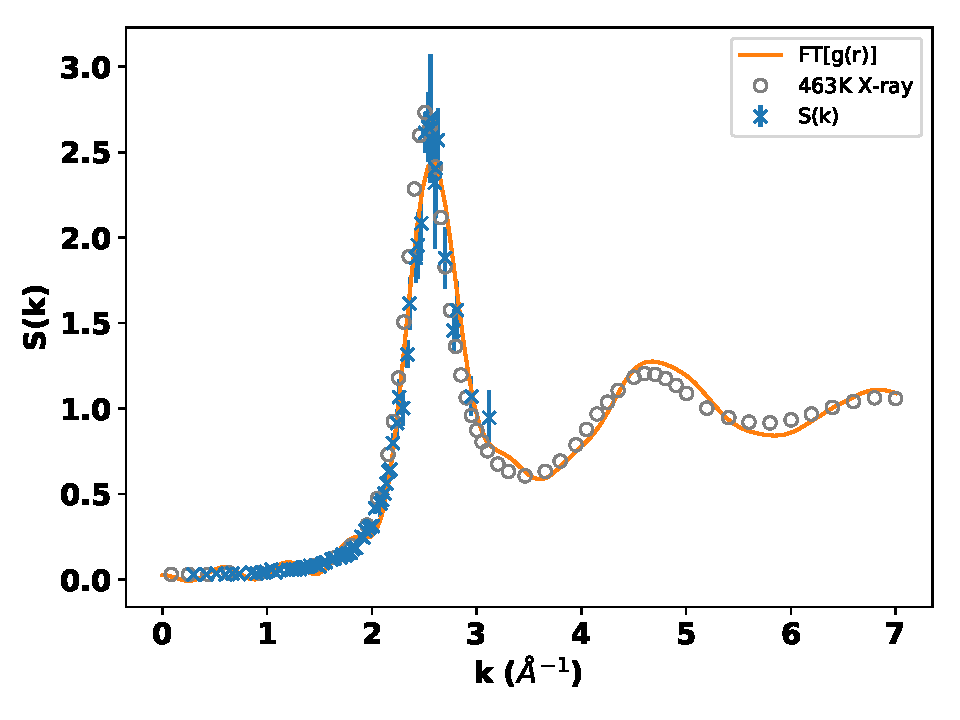
\includegraphics[scale=0.48]{figures/009d_amass-cont1_t500}
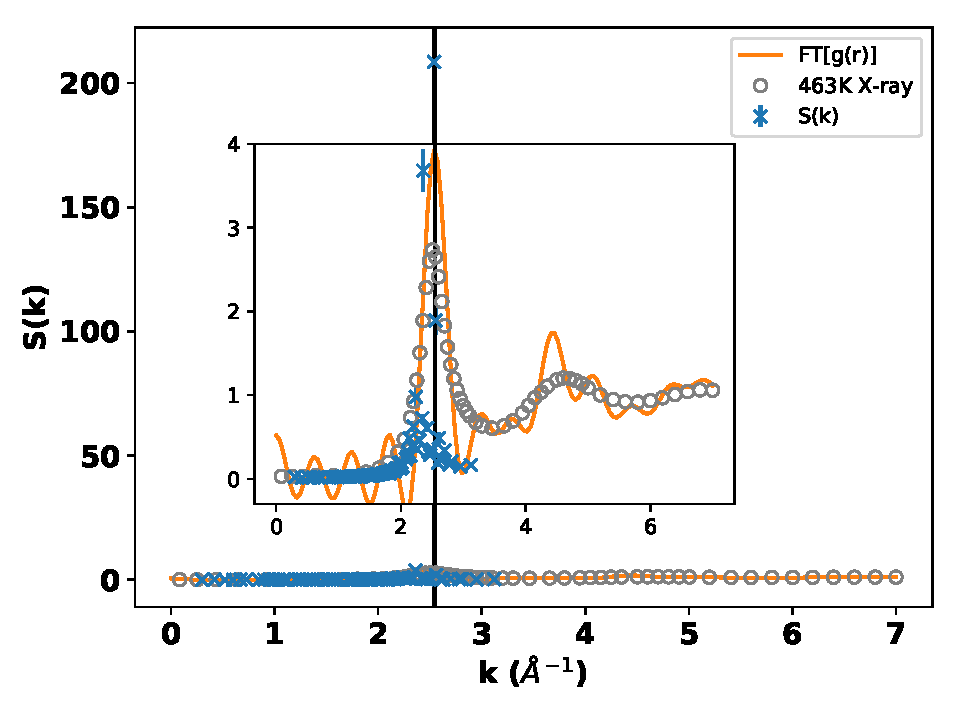
\includegraphics[scale=0.48]{figures/009d_amass-temp330}
\caption{Structure factor of disordered lithium configurations in liquid (left) and solid (right) phases. 32 lithium configurations were generated in each phase. Each configuration contained 432 lithium atoms in a cubic box with side length 20.96$\AA$. The liquid configurations were generated at $T=500K$, whereas the solid configurations were generated at $T=330K$. The blue crosses are spherically-averaged $S(k)$ calculated directly in reciprocal space. The solid line is the Fourier transform of the real-space pair correlation function $g(r)$. The gray circles are experimental values from X-ray scattering~\cite{Waseda1981,Mokshin2018}.}
\label{fig:lisk}
\end{figure}

\subsection{QMC Energies}

The orbitals in the Slater determinant were obtained using KS-LDA. We used a planewave cutoff of 256 Ry in the all-electron calculation. The resultant orbitals were modified to remove the approximate electron-ion cusp, which is exactly re-introduced in the Jastrow. All pseudopotential calculations used the BFD pseudopotential and a planewave cutoff of 16 Ry.

QMC calculations were carried out at valence density $r_s=3.25$, consistent with the previous study~\cite{Filippi1999}. 
QMC energies of the all-electron simulations are shown in the first three rows of Table~\ref{tab:qmc-etv}. Timestep error is $\sim$ 3 mha/e/a.u.. Mixed-estimator error of the kinetic energy is $\sim$ 10 mha/e. These errors are larger than their pseudopotential counterparts. Nevertheless, our DMC total energy of -2.5142 ha/e is within 1.5 mha/e of the -2.5129 ha/e obtained in a previous QMC study using localized basis and the PBE functional~\cite{Rasch2015}. The previous study was performed at a valence density of $r_s=3.24$, which is very close to our $r_s=3.25$.
Energies from the pseudopotential simulations are shown in the remaining rows of Table~\ref{tab:qmc-etv}. The difference between pseudopotential DMC and VMC total energies are consistently around 1 mha/e. Further, the timestep error is $\sim$ 0.1 mha/e/a.u. and the mixed-estimator error of the kinetic energy is $<$ 1 mha/e. These small differences verify the high quality of our trial wavefunction for the valence electrons.

\begin{table}[h]
\begin{tabular}{rrrllllll}
\toprule
 $N_e/N_{Li}$ &  Classical T &  $\langle N_e\rangle$ & method & timestep &    acc & $\langle E\rangle/\langle N_e\rangle$ & $\sigma_E^2/\langle N_e\rangle$ & $\langle T\rangle/\langle N_e\rangle$ \\
\midrule
            3 &            0 &                161.93 &    VMC &      0.8 &  43.51 &                           -2.51036(2) &                       0.0204(2) &                              2.506(2) \\
            3 &            0 &                161.93 &    DMC &     0.01 &  98.79 &                           -2.51413(1) &                      0.01888(2) &                             2.5097(4) \\
            3 &            0 &                161.93 &    DMC &    0.005 &  99.53 &                           -2.51416(1) &                      0.01890(2) &                             2.5098(3) \\
            1 &            0 &                 54.11 &    VMC &        2 &  81.88 &                           -0.25573(3) &                      0.00393(4) &                            0.15076(7) \\
            1 &            0 &                 54.11 &    DMC &      0.2 &   98.7 &                           -0.25709(1) &                      0.00432(2) &                            0.14974(3) \\
            1 &            0 &                 54.11 &    DMC &      0.1 &  99.47 &                          -0.256986(8) &                      0.00421(1) &                            0.14985(3) \\
            1 &            0 &                431.41 &    VMC &     3.25 &  71.64 &                          -0.254517(3) &                     0.004173(9) &                           0.150858(8) \\
            1 &            0 &                431.41 &    DMC &      0.2 &   98.7 &                          -0.255730(4) &                     0.004631(8) &                            0.15025(2) \\
            1 &            0 &                431.41 &    DMC &      0.1 &  99.47 &                          -0.255630(4) &                     0.004518(7) &                            0.15032(2) \\
            1 &          330 &                431.85 &    VMC &        3 &  73.91 &                        -0.2520480(10) &                     0.004274(3) &                           0.152858(3) \\
            1 &          330 &                431.85 &    DMC &      0.3 &  97.85 &                         -0.2534085(9) &                     0.004872(2) &                           0.152212(3) \\
            1 &          330 &                431.85 &    DMC &     0.15 &  99.11 &                         -0.2532710(9) &                     0.004803(2) &                           0.152279(3) \\
            1 &          500 &                431.90 &    VMC &        3 &  73.54 &                          -0.249699(1) &                     0.004383(3) &                           0.154636(3) \\
            1 &          500 &                431.90 &    DMC &      0.3 &  97.81 &                         -0.2511151(9) &                     0.005000(2) &                           0.154009(3) \\
            1 &          500 &                431.90 &    DMC &     0.15 &  99.09 &                         -0.2509826(9) &                     0.004937(2) &                           0.154079(3) \\
\bottomrule
\end{tabular}

\caption{QMC energies and variance. All energies are reported in ha/e. Variance is in ha$^2$/e. Timestep is in ha$^{-1}$. Monte Carlo acceptance rate (acc) is in percent.\label{tab:qmc-etv}}
\end{table}


\subsection{QMC Electronic Structure Factor}

The fluctuating electronic structure factor
\begin{align}
\delta S(k) \equiv \left\langle
(\rho_{\bs{k}}-\bar{\rho}_{\bs{k}})^* (\rho_{\bs{k}}-\bar{\rho}_{\bs{k}})
\right\rangle,
\end{align}
where $\rho_{\bs{k}} = \sum\limits_j^{N_e} e^{i\bs{r}_j\cdot\bs{k}}$ is the collective coordinate of the electrons. The $\braket{}$ denotes expectation value, and $\bar{\rho}_{\bs{k}}\equiv\braket{\rho}_{\bs{k}}$. The QMC fluctuating structure factors are shown in Fig.~\ref{fig:qmc-dsk}. All values are linearly extrapolated to remove the mixed-estimator bias. The pseudopotential $\delta S(k)$ is insensitive to disorder. The $\delta S(k)$ from 432-atom simulations of perfect crystal, disordered solid, and liquid structures are indistinguishable from one another. Further, finite system size has only a small effect on the electronic structure factor, because the $\delta S(k)$ of the 54-atom simulation is very close to the 432-atom one. All pseudopotential $\delta S(k)$ can be accurately described by the RPA $S(k)$ at the same valence density when $k<0.4$ a.u.. Our all-electron structure factor agrees well with that from the previous QMC study [Rasch2015].

\begin{figure}[h]
%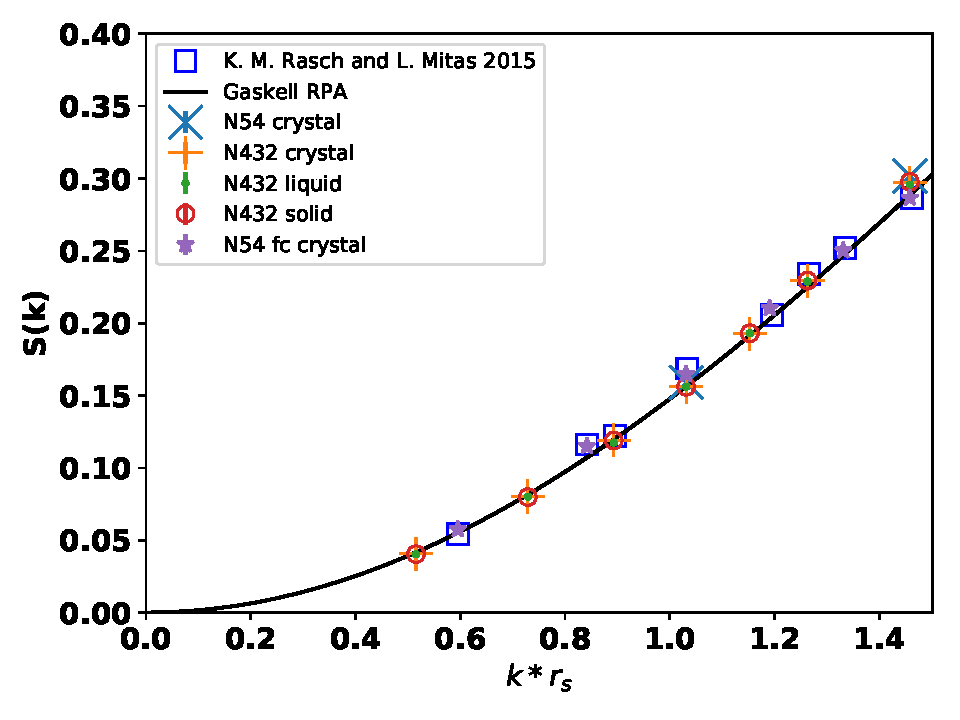
\includegraphics[scale=0.6]{figures/li40bg_dsk-bfd-fc}
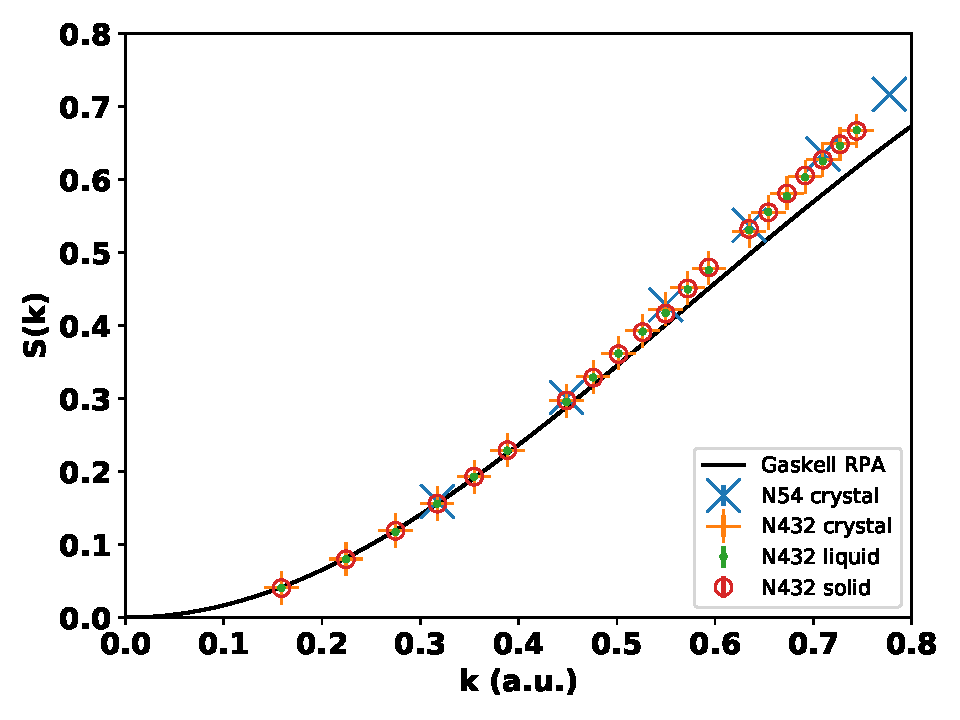
\includegraphics[width=0.48\linewidth]{figures/li40bg_dsk-bfd}
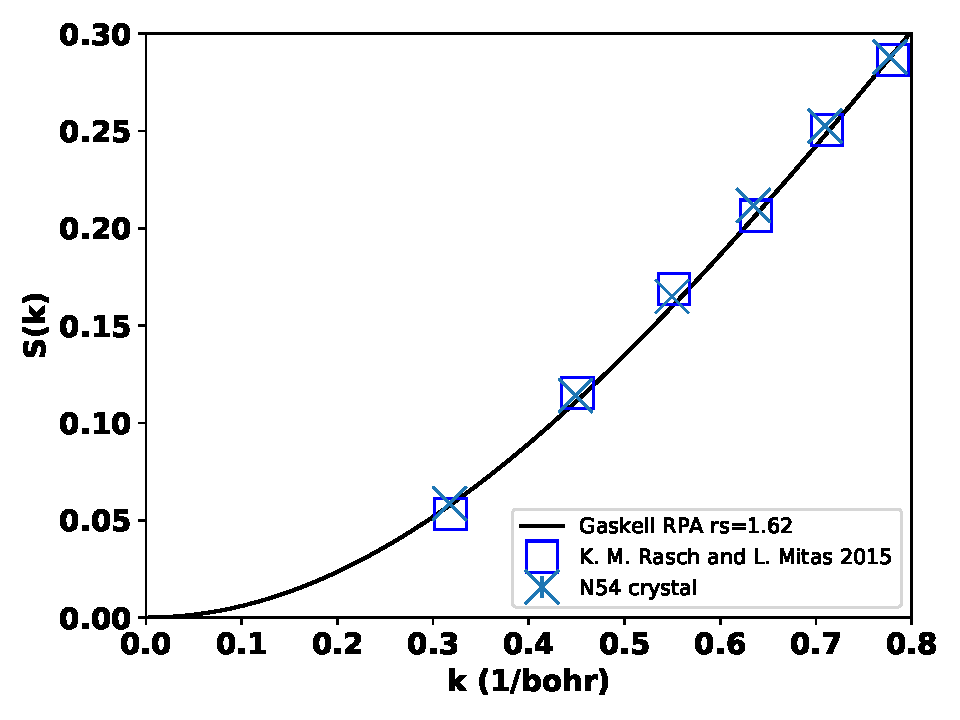
\includegraphics[width=0.48\linewidth]{figures/li40bg_dsk-fc}
\caption{Electronic static structure factor of pseudopotential (left) and all-electron (right) QMC simulations in 54-atom and 432-atom simulation cells. The black line in the left plot is RPA $S(k)$ at valence density $r_s=3.25$. It fits lithium valence $S(k)$ remarkably well for $k<0.4 a.u.$. In the right plot, the black line is RPA $S(k)$ at density $r_s=3.25/\sqrt{3}$. \label{fig:qmc-dsk}}
\end{figure}


\subsection{QMC Momentum Distribution}

The momentum distribution is obtained on a cubic regular grid with spacing $dk=0.040$ a.u. in reciprocal space. To achieve this grid spacing, uniform twist-average grids of size $8^3$ and $4^3$ are used in the 54-atom and 432-atom simulations, respectively. The twist-average grid is either $\Gamma$-centered or shifted by $dk/2$ in all directions. In the perfect crystal, cubic symmetries reduce the number of unique twists from 64 to 4 and 512 to 20 on a shifted grid, and 64 to 10 and 512 to 35 on a $\Gamma$-centered grid. The reciprocal-space grid is truncated at a spherical cutoff of $1.49$ a.u. in the solid and liquid simulations.
%The tail of the momentum distribution is extended to at least $3.0$ a.u. in post-processing.
%in 1/48th of the cubic reciprocal space, representing the irreducible wedge. The results are unfolded using cubic symmetries onto a regular grid with a spherical cutoff.

A QMC Compton profile is computed in four steps. First, the 3D DMC $n(\bs{k})$ is linearly extrapolated to reduce the mixed-estimator bias using VMC data. Second, the linearly-extrapolated $n(\bs{k})$ is spherically averaged to obtain a 1D distribution $n(k)$. Third, the 1D $n(k)$ is extended to large k by fitting the tail region ($k > 1.2$ a.u.) of QMC $n(k)$ to a model function eqn.~(\ref{eq:nktail}), which is inspired by the momentum distribution of hydrogen-like atoms
\begin{align} \label{eq:nktail}
n_{tail}(k, A, Z) = A\left(\dfrac{2Z}{(k^2+Z^2)^2}\right)^2,
\end{align}
where $A$ and $Z$ are fitting parameters. Fourth and finally, the 1D $n(k)$ is integrated to obtain the spherically-averaged Compton profile $J(p)$ via eqn.~(\ref{eq:jp1d}) and split into two parts at a cutoff momentum $k_c$
\begin{align} \label{eq:jp1d}
J(p) = \left( \dfrac{(2\pi)^3}{\Omega/N_{Li}} \right)\left[
\int\limits_p^{k_c} k n(k) dk + \int\limits_{k_c}^{\infty} k n_{tail}(k, A^*, Z^*) dk
\right],
\end{align}
where $\Omega$ is the volume of the supercell, $N_{Li}$ is the number of lithium atoms in the supercell, and $A^*$, $Z^*$ are chosen to satisfy momentum distribution sum rules. %The prefactor is needed because $n(\bs{k})$ in simulation is scaled by reciprocal volume and is always in the range [0, 2].
The sum-rules of the momentum distribution and the Compton profile in our convention are
\begin{align}
\left( \dfrac{(2\pi)^3}{\Omega/N_{Li}} \right)^{-1} \int d\bs{k} n(\bs{k}) =& \braket{N_e}/N_{Li}, \label{eq:nsum} \\
\left( \dfrac{(2\pi)^3}{\Omega/N_{Li}} \right)^{-1} \int d\bs{k} n(\bs{k})~\frac{\hbar^2k^2}{2m_e} =& \braket{T}/N_{Li}, \label{eq:tsum} \\
\int_{-\infty}^{\infty} dp J(p) =& \braket{N_e}/N_{Li}, \label{eq:jpsum}
\end{align}
where $\braket{T}$ is the expectation value of the total kinetic energy. We find it important to extend the tail of $n(k)$ so that it satisfies the sum rules. The fitted values in the tail function eqn.~(\ref{eq:nktail}) are shown in Tables~\ref{tab:crystal-ntsum}-\ref{tab:fc-ntsum}, along with sum-rule compliance. The normalization sum rule eqn.~(\ref{eq:nsum}) is labeled ``nsum''. The kinetic energy sum rule eqn.~(\ref{eq:tsum}) is labeled ``tsum''.

\begin{table}[h]
\caption{Perfect crystal spherically-averaged momentum distribution sum rules and tail. \label{tab:crystal-ntsum}}
\begin{subtable}{0.49\textwidth}
% li40_bfd-1/li6a/gcta.py
% li40_bfd-4/target_kglue/glue_tail.py
\caption{BCC Crystal BFD N54 $n(k)$ sum rules with and without extended tail.\label{tab:solid-bfd-n54-sum02}}
\begin{tabular}{cclllll}
\toprule
method & kcut & nsum & tsum & texpect & A & Z \\
\midrule
VMC & 1.57 & 1.001 & 0.1407 \\
DMC & 1.57 & 1.002 & 0.1397 \\
lin. ex. & 1.57 & 1.003 & 0.1387 \\
VMC & 80.0 & 1.007 & 0.1518 & 0.15242(6) & 0.06 & 0.40 \\
DMC & 80.0 & 1.007 & 0.1486 & 0.15006(4) & 0.06 & 0.35 \\
lin. ex. & 80.0 & 1.006 & 0.1457 & 0.14771(8) & 0.07 & 0.30 \\
\bottomrule
\end{tabular}
\end{subtable}
\begin{subtable}{0.49\textwidth}
% li40_bfd-1/li6b/gcta.py
% li40_bfd-4/target_kglue/glue_tail.py
\caption{BCC Crystal BFD N432 $n(k)$ sum rules with and without extended tail.\label{tab:solid-bfd-n432-sum02}}
\begin{tabular}{ccllll}
\toprule
method & kcut & nsum & tsum & A & Z \\
\midrule
VMC & 1.5 & 0.992 & 0.1372 \\
DMC & 1.5 & 0.992 & 0.1370 \\
lin. ex. & 1.5 & 0.992 & 0.1368 \\
VMC & 80.0 & 0.997 & 0.1465 & 0.10 & 0.26 \\
DMC & 80.0 & 0.997 & 0.1459 & 0.13 & 0.22 \\
lin. ex. & 80.0 & 0.997 & 0.1453 & 0.18 & 0.18 \\ 
\bottomrule
\end{tabular}
\end{subtable}
\end{table}

\begin{table}[h]
\caption{Disordered configurations spherically-averaged momentum distribution sum rules and tail. \label{tab:conf-ntsum}}
\begin{subtable}{0.49\textwidth}
\caption{Solid configuration BFD N432 $n(k)$ sum rules with and without extended tail.\label{tab:solid-conf31-bfd-n432-sum02}}
\begin{tabular}{ccllll}
\toprule
method & kcut & nsum & tsum & A & Z \\
\midrule
VMC & 1.5 & 0.991 & 0.1379 & \\
DMC & 1.5 & 0.991 & 0.1380 & \\
lin. ex. & 1.5 & 0.991 & 0.1380 & \\
VMC & 80.0 & 0.998 & 0.1503 & 0.049 & 0.465 \\
DMC & 80.0 & 0.998 & 0.1504 & 0.048 & 0.465 \\
lin. ex. & 80.0 & 0.998 & 0.1504 & 0.048 & 0.464\\
\bottomrule
\end{tabular}
\end{subtable}
\begin{subtable}{0.49\textwidth}
\caption{Liquid BFD N432 $n(k)$ sum rules with and without extended tail.\label{tab:liquid-bfd-n432-sum02}}
\begin{tabular}{ccllll}
\toprule
method & kcut & nsum & tsum & A & Z \\
\midrule
VMC & 1.5 & 0.991 & 0.1385 & \\
DMC & 1.5 & 0.992 & 0.1392 & \\
lin. ex. & 1.5 & 0.993 & 0.1400 & \\
VMC & 80.0 & 0.999 & 0.1539 & 0.04 & 0.57 \\
DMC & 80.0 & 1.000 & 0.1556 & 0.04 & 0.60 \\
lin. ex. & 80.0 & 1.002 & 0.1582 & 0.04 & 0.65\\
\bottomrule
\end{tabular}
\end{subtable}
\end{table}

\begin{table}[h]
\caption{All-electron crystal spherically-averaged momentum distribution sum rules and tail. \label{tab:fc-ntsum}}
\begin{subtable}{0.49\textwidth}
% li40_fc-4/target_kglue/glue_tail.py
\caption{BCC crystal full-core N54 $n(k)$ sum rules with and without extended tail.\label{tab:solid-bare-n54-sum02}}
\begin{tabular}{cclllll}
\toprule
method & kcut & nsum & tsum & texpect & A & Z \\
\midrule
VMC & 3.0 & 0.858 & 0.9000 \\
DMC & 3.0 & 0.854 & 0.9032 \\
lin. ex. & 3.0 & 0.850 & 0.9064 \\
VMC & 80.0 & 1.002 & 2.4359 & 2.487(6) & 13.5 & 2.76 \\
DMC & 80.0 & 1.000 & 2.4392 & 2.4982(3) & 13.5 & 2.76 \\
lin. ex. & 80.0 & 0.997 & 2.4420 & 2.510(6) & 13.5 & 2.77 \\
\bottomrule
\end{tabular}
\end{subtable}
\end{table}

\bibliographystyle{apsrev4-1}
\bibliography{ref}

\end{document}
